\chapter{curriculum vitae}

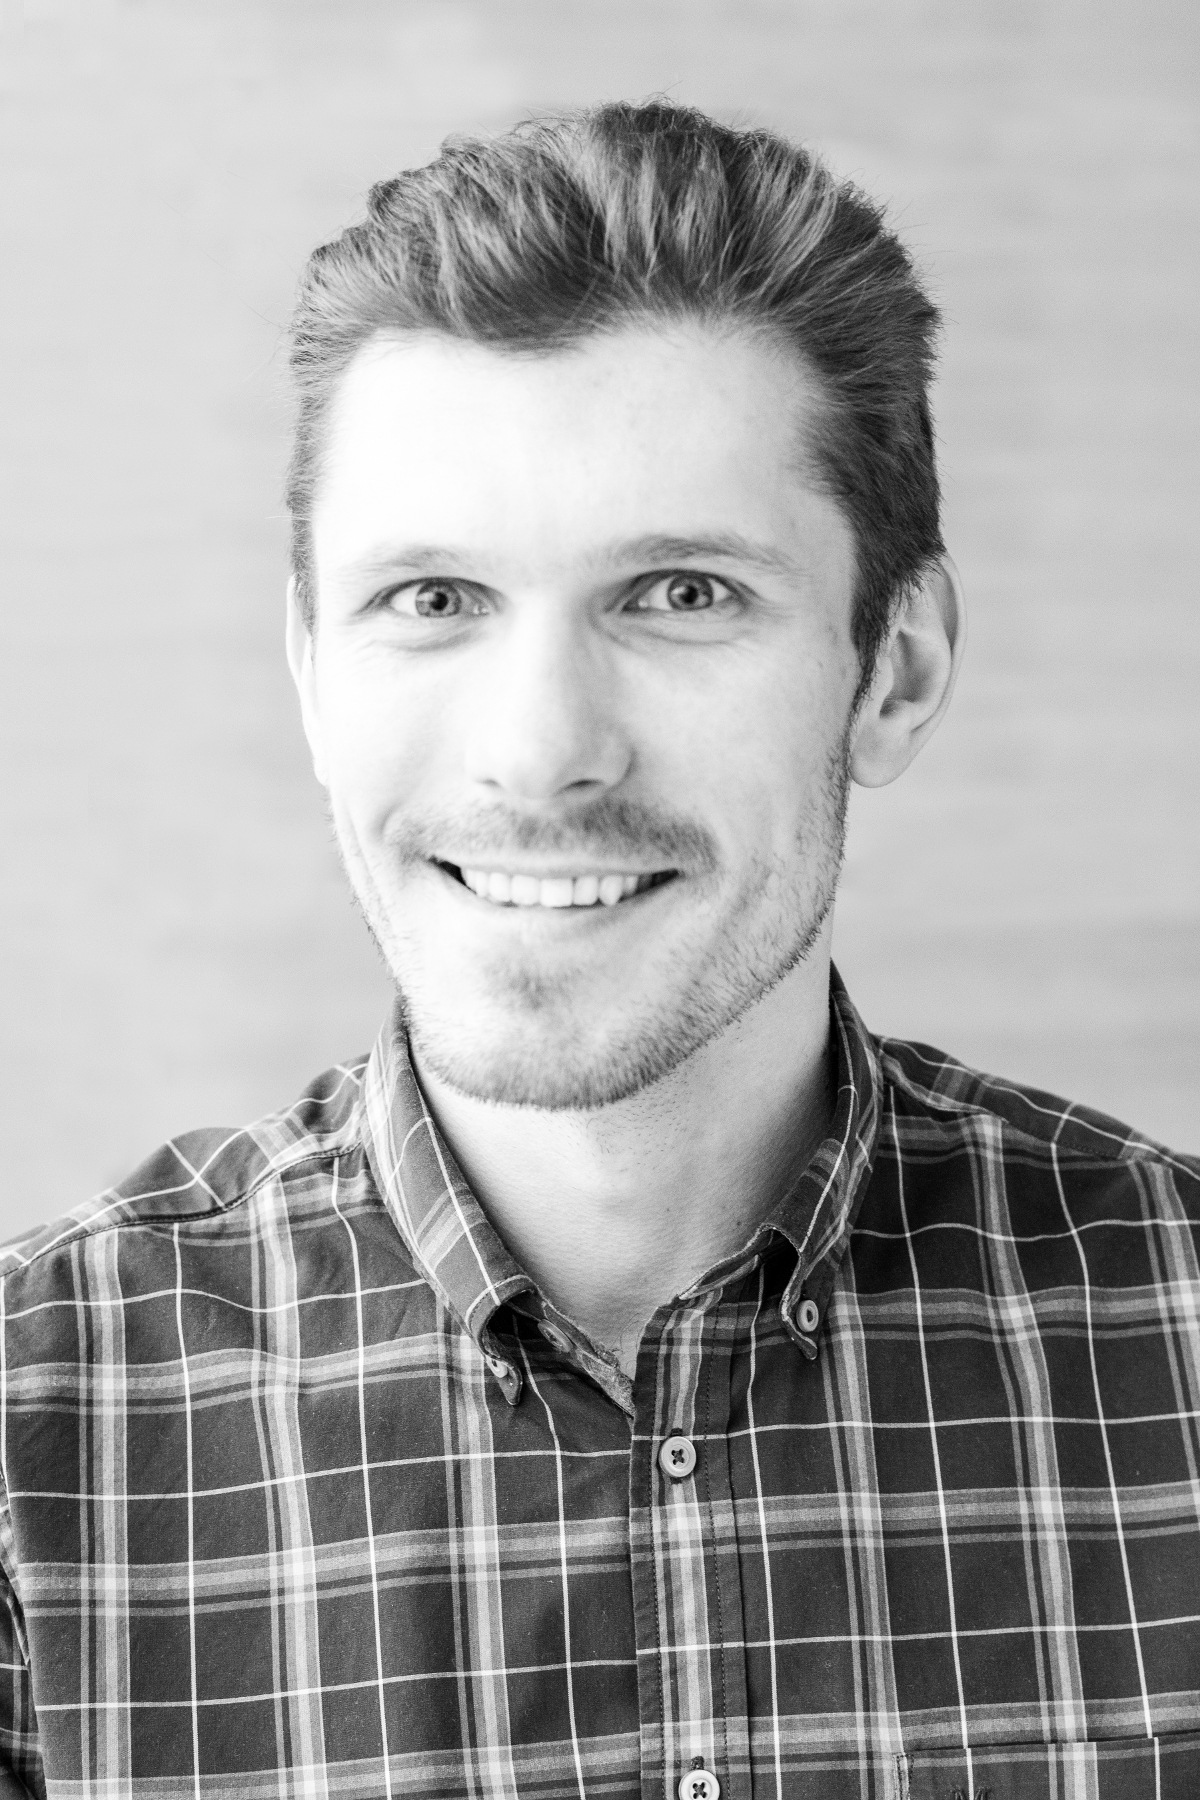
\includegraphics[width=30mm]{assets/me.jpg}

\textbf{PhD in Neurobiology}\\
Research study: Impact of different sensory conditions on the hippocampal population code for space (in-vivo electrophysiology)\\
Cognition and Neural Plasticity, Ludwig-Maximilians-Universität Munich\\
Supervisors: Prof. Dr. Christian Leibold, Prof. Dr. Anton Sirota

\textbf{Software Developer, German Neuroinformatics Node}\\
Development of tools for handling/analyzing neurophysiological data.\\
Computational Neuroscience, Ludwig-Maximilians-Universität Munich\\
Supervisor: Prof. Dr. Thomas Wachtler. Projects: https://github.com/G-Node

\textbf{Systems Analyst / Programmer}\\
Industry assignments for General Motors Europe and Philip Morris International

\textbf{Post-graduate study, Computational Modelling}\\
Department of Design and Analysis of Oil Field Development\\
Russian Oil and Gas Scientific Research Institute

\textbf{Diploma in Applied Mathematics and Computer Science}\\
Department of Computational Mathematics and Cybernetics\\
Moscow State University of M.V. Lomonosov\\
Qualification: mathematician / systems programmer\\
Specification: applied mathematics and informatics



\chapter{List of publications}

\underline{First author:}

\textbf{Sobolev, A.}, Stoewer, A., Leonhardt, A., Rautenberg, P. L., Kellner, C. J., Garbers, C., \& Wachtler, T. (2014). Integrated platform and API for electrophysiological data. Frontiers in Neuroinformatics, 8(APR).
%https://doi.org/10.3389/fninf.2014.00032

\textbf{Sobolev, A.}, Stoewer, A., Leonhardt, A., Rautenberg, P. L., Kellner, C. J., Garbers, C., \& Wachtler, T. (2014). Integrated platform and API for electrophysiological data. Frontiers in Neuroinformatics, 8(APR).
%https://doi.org/10.3389/fninf.2014.00032

\underline{co-author:}

Ferreiro, D. N., Amaro, D., Schmidtke, D., \textbf{Sobolev, A.}, Gundi, P., Belliveau, L., Sirota, A., Grothe, B., \& Pecka, M. (2020). Sensory Island Task (SIT): A New Behavioral Paradigm to Study Sensory Perception and Neural Processing in Freely Moving Animals. Frontiers in Behavioral Neuroscience, 14.
%https://doi.org/10.3389/fnbeh.2020.576154

Zehl, L., Jaillet, F., Stoewer, A., Grewe, J., \textbf{Sobolev, A.}, Wachtler, T., Brochier, T. G., Riehle, A., Denker, M., \& Grün, S. (2016). Handling metadata in a neurophysiology laboratory. Frontiers in Neuroinformatics, 10(JUL).
%https://doi.org/10.3389/fninf.2016.00026

Garcia, S., Guarino, D., Jaillet, F., Jennings, T., Pröpper, R., Rautenberg, P. L., Rodgers, C. C., \textbf{Sobolev, A.}, Wachtler, T., Yger, P., \& Davison, A. P. (2014). Neo: An object model for handling electrophysiology data in multiple formats. Frontiers in Neuroinformatics, 8(FEB).
%https://doi.org/10.3389/fninf.2014.00010

Rautenberg, P. L., \textbf{Sobolev, A.}, Herz, A. V. M., \& Wachtler, T. (2011). A database system for electrophysiological data. In Lecture Notes in Computer Science (including subseries Lecture Notes in Artificial Intelligence and Lecture Notes in Bioinformatics): Vol. 6990 LNCS.
%https://doi.org/10.1007/978-3-642-23740-9



\chapter{Affidavit}
Hiermit versichere ich an Eides statt, dass ich die vorliegende Dissertation "Contribution of the idiothetic and the allothetic information to the hippocampal place code" selbstständig angefertigt habe, mich außer der angegebenen keiner weiteren Hilfsmittel bedient und alle Erkenntnisse, die aus dem Schrifttum ganz oder annähernd übernommen sind, als solche kenntlich gemacht und nach ihrer Herkunft unter Bezeichnung der Fundstelle einzeln nachgewiesen habe.

I hereby confirm that this dissertation "Contribution of the idiothetic and the allothetic information to the hippocampal place code" is the result of my own work and that I have only used sources or materials listed and specified in the dissertation.


\vspace{0.3in}

\noindent Munich, \today

\vspace{1in}

\noindent Andrey Sobolev


\chapter{Author Contributions}
Andrey Sobolev, Dr. Kay Thurley, Dr. Dustin Fetterhoff, Prof. Dr. Christian Leibold and Prof. Dr. Anton Sirota contributed to this research study.

The project was established by Anton Sirota, Christian Leibold and Kay Thurley. The design of the experimental protocols and the virtual environment was done by Andrey Sobolev with the support of Anton Sirota. Animal handling was performed by Andrey Sobolev under the guidance of Kay Thurley. Printing and assembling implants as well as the surgical procedures were done by Andrey Sobolev. Dustin Fetterhoff contributed with animals from his project to the study. Data analysis was done by Andrey Sobolev under review of Anton Sirota and Christian Leibold.

We assert that aforementioned author contributions are correct and accurate:

\vspace{0.3in}

\noindent Munich, \today

\vspace{0.8in}

\noindent Andrey Sobolev

\vspace{0.8in}

\noindent Prof. Dr. Anton Sirota
